\documentclass[/home/jesse/Analysis/FemtoAnalysis/AnalysisNotes/AnalysisNoteJBuxton.tex]{subfiles}

\renewcommand{\NonFlatBgdLamKch}{_NonFlatBgdCrctnPolynomial}
\renewcommand{\NonFlatBgdLamKs}{_NonFlatBgdCrctnLinear}

\renewcommand{\ResNum}{_NoRes}

\renewcommand{\SaveNameModLamKch}{\MomRes\NonFlatBgdLamKch\ResNum\ParamFixAndShareLamKch}
\renewcommand{\SaveNameModLamKs}{\MomRes\NonFlatBgdLamKs\ResNum\ParamFixAndShareLamKs}

\begin{document}

\subsubsection{Results: \LamKs and \LamKpm: No Residual Correlations Included in Fit}
\label{ResultsLamK_NoRes}

Figure \ref{fig:ScattParams_NoRes} nicely collects and summarizes all of our extracted fit parameters for the case of no included residual contributors.  Figure \ref{fig:mTScalingOfRadii_NoRes} presents our extracted fit radii, along with those of other systems previously analyzed by ALICE \cite{Adam:2015vja}, as a function of pair transverse mass (\mt).
Figures \ref{fig:LamK0wConjFits_NoRes}, \ref{fig:LamKchPwConjFits_NoRes}, and \ref{fig:LamKchMwConjFits_NoRes} show the experimental correlation functions with fits, assuming no residual contributors, for all studied centralities for \LamKs with \ALamKs, \LamKchP with \ALamKchM, and \LamKchM with \ALamKchP, respectively.
The parameter sets extracted from the fits can be found in Tables \ref{tab:FitResultsLamK0_3Res} and \ref{tab:FitResultsLamKch_3Res}.


\begin{figure}[h]
  \centering
  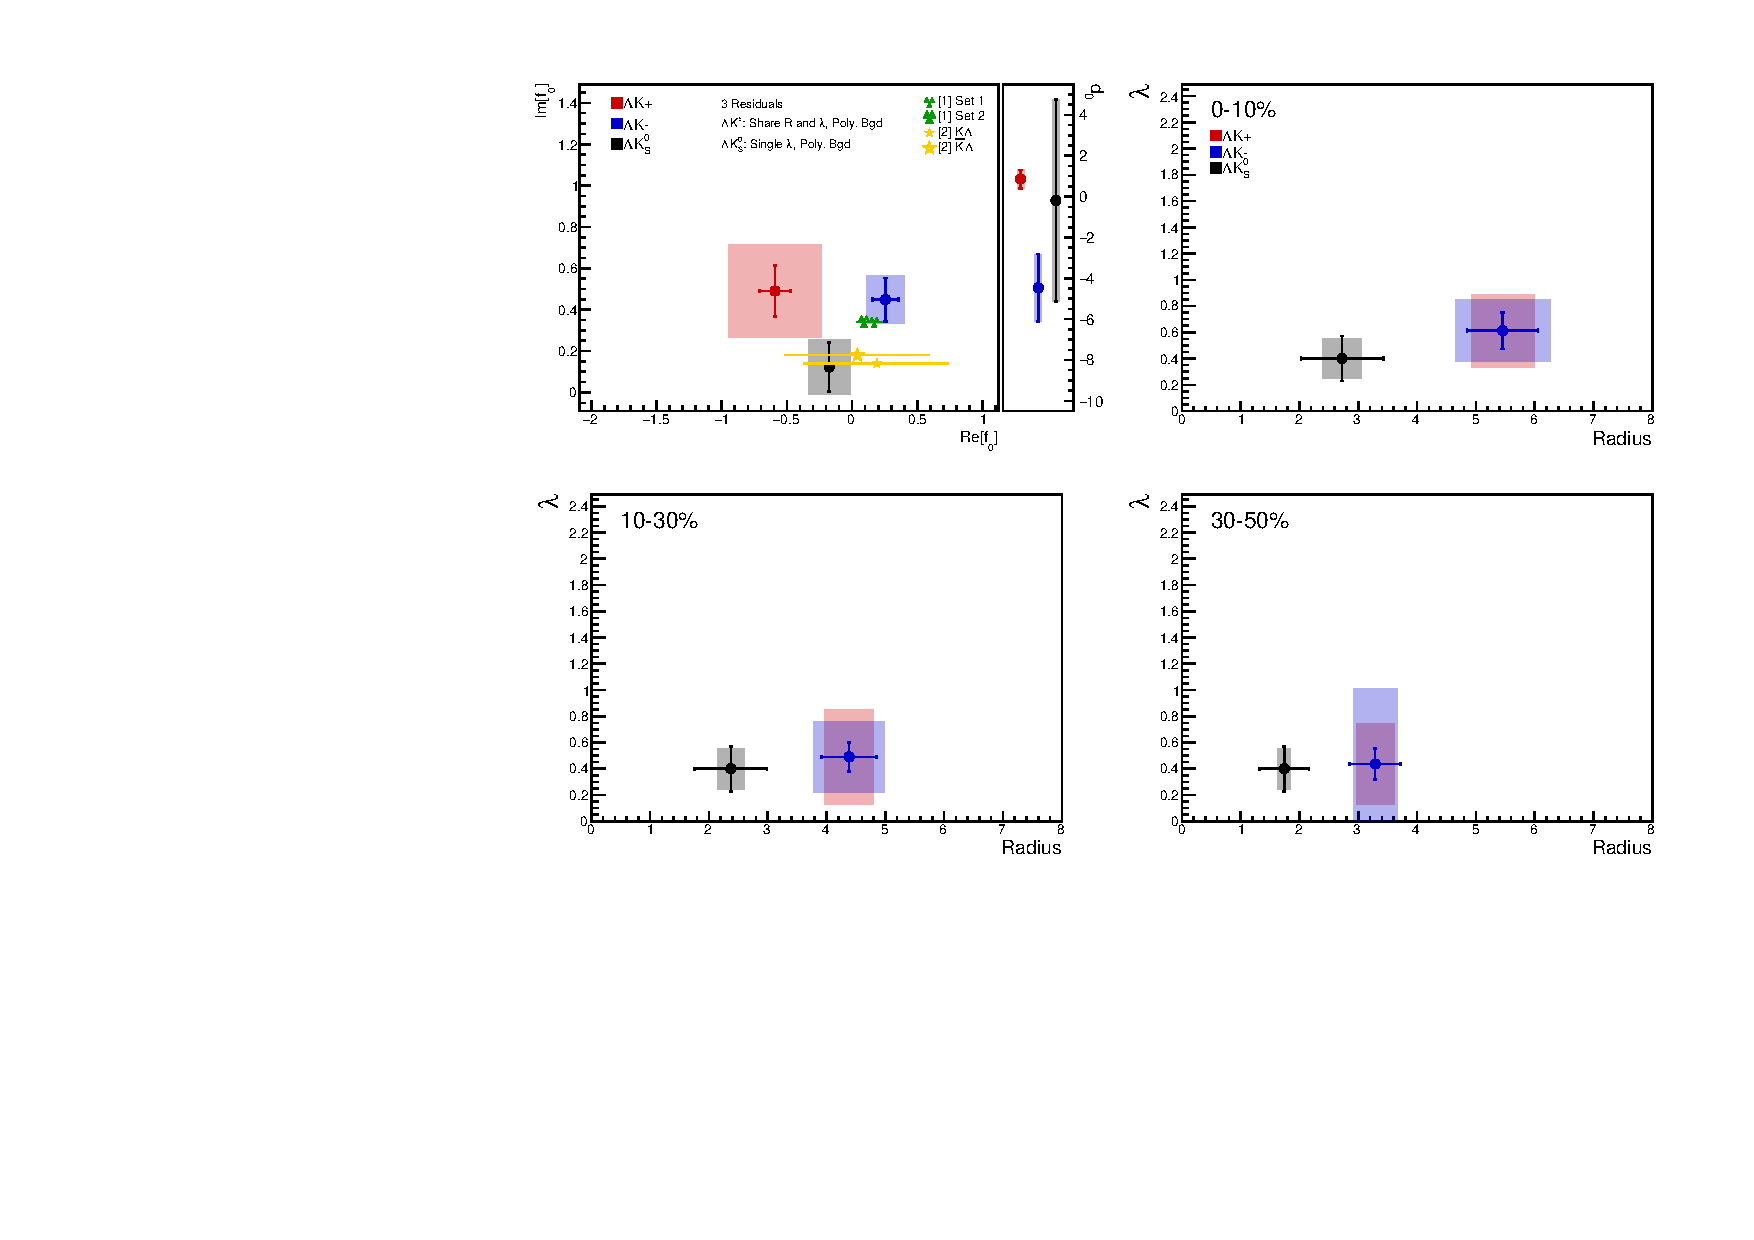
\includegraphics[width=0.80\textwidth]{7_ResultsAndDiscussion/Figures/CompareAllScattParams_Comp3An_NoRes.pdf}
  \caption[Extracted Scattering Parameters: No Residuals in Fit]{Extracted scattering parameters for the case of NO residual contributors for all of our $\Lambda$K systems.  [Top Left]: $\mathbb{I}f_{0}$ vs. $\mathbb{R}f_{0}$, together with d$_{0}$ to the right.  [Top Right (Bottom Left, Bottom Right)]: $\lambda$ vs. Radius for the 0-10\% (10-30\%, 30-50\%) bin.  The green \cite{Liu:2006xja} and yellow \cite{Mai:2009ce} points show theoretical predictions made using chiral perturbation theory.}
  \label{fig:ScattParams_NoRes}
\end{figure}



Figure \ref{fig:mTScalingOfRadii_NoRes} shows extracted $R_{\mathrm{inv}}$ parameters as a function of tranverse mass ($m_{\mathrm{T}}$) for various pair systems over several centralities.  The published ALICE data \cite{Adam:2015vja} is shown with transparent, open symbols.  The new $\Lambda$K results are shown with opaque, filled symbols.  The radii shown an increasing size with increasing centrality, as is expected from the simple geometric picture of the collisions.  The radii decrease in size with increasing $m_{\mathrm{T}}$, and we see an approximate scaling of the radii with transverse mass, as is expected in the presence of collective flow in the system.

\begin{figure}[h]
  \centering
  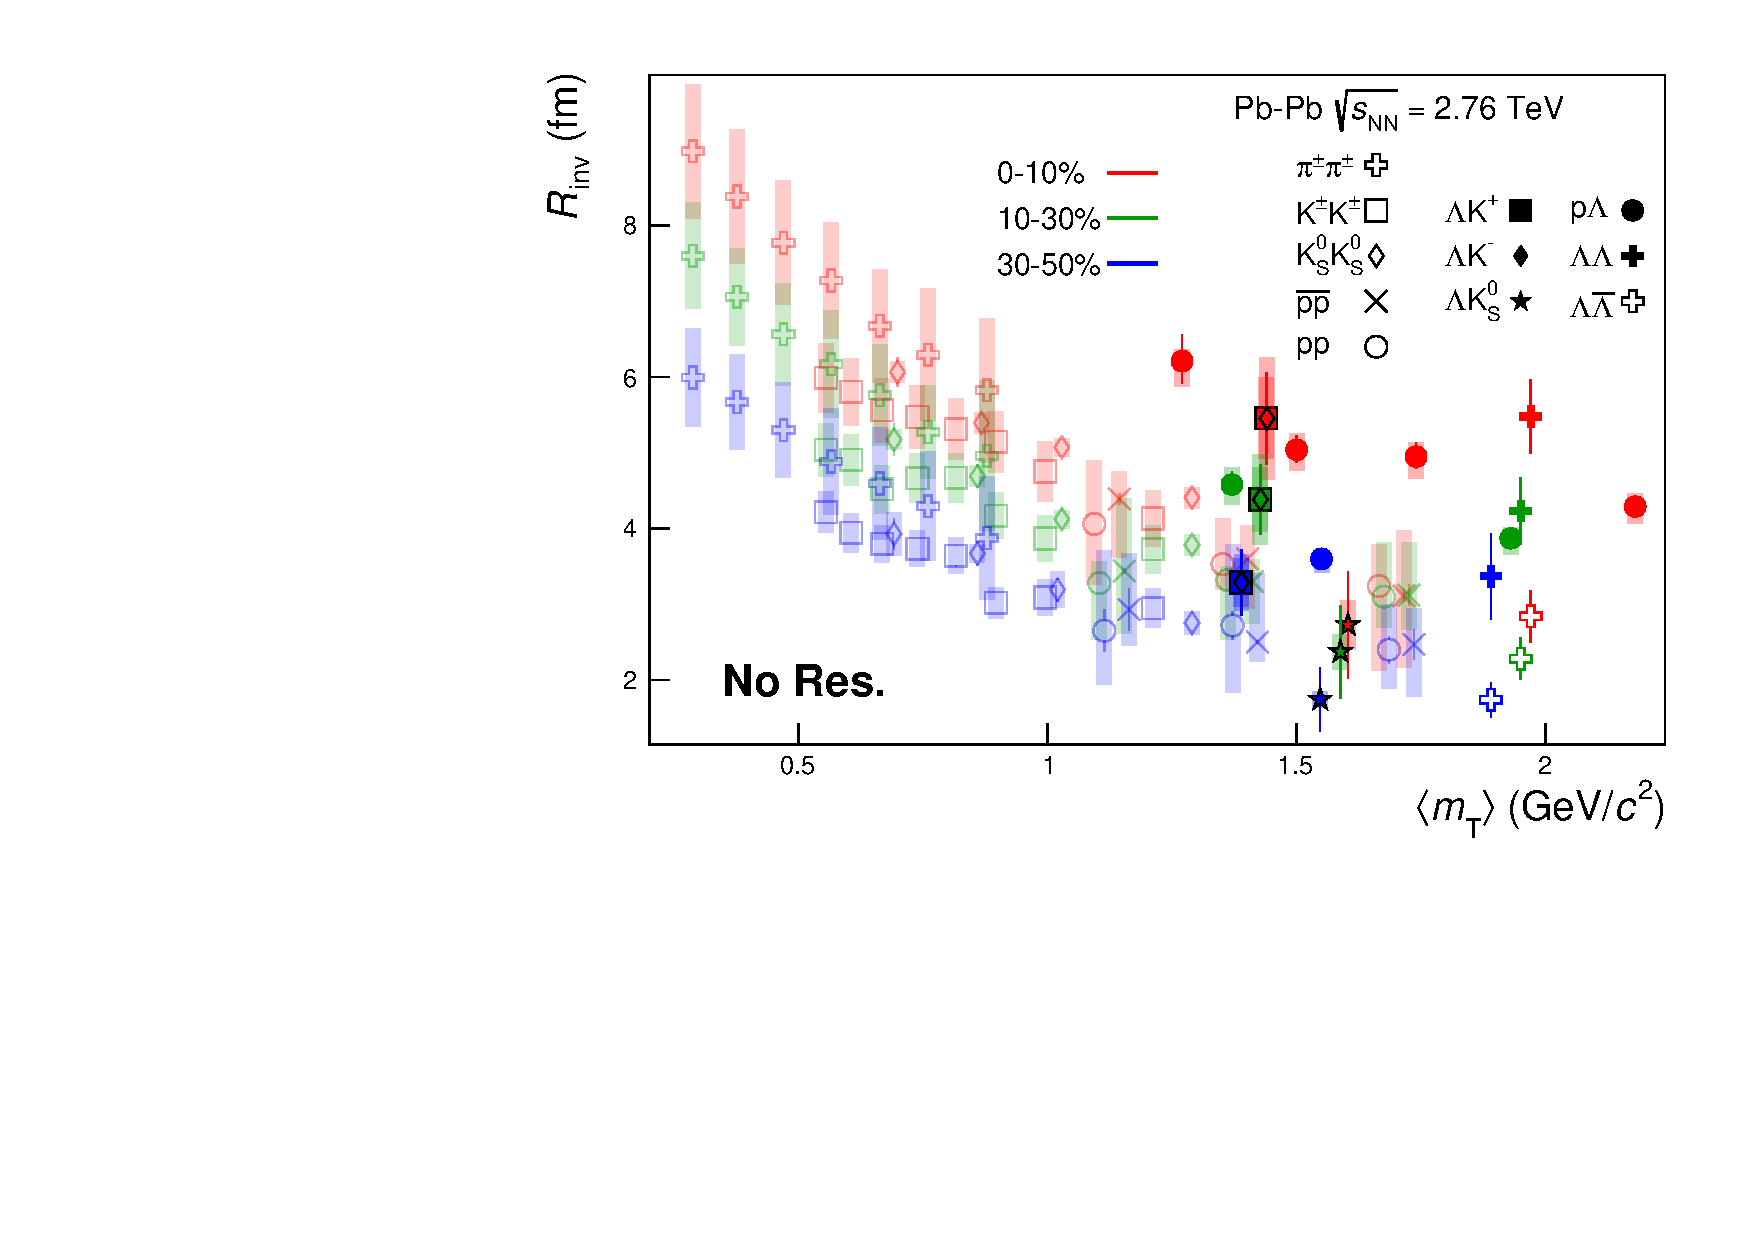
\includegraphics[width=0.50\textwidth]{7_ResultsAndDiscussion/Figures/mTscaling_MinvCalc_OutlinedPoints_OthersTransparent_wJaiAndHans_NoRes.pdf}
  \caption[$m_{\mathrm{T}}$ Scaling of Radii: No Residuals in Fit]{No residual correlations in $\Lambda$K fits.  Extracted fit $R_{\mathrm{inv}}$ parameters as a function of pair transverse mass ($m_{\mathrm{T}}$) for various pair systems over several centralities. The ALICE published data \cite{Adam:2015vja} is shown with transparent, open symbols.  The new $\Lambda$K results are shown with opaque, filled symbols.  In the left, the $\Lambda$K$^{+}$ (with it's conjugate pair) results are shown separately from the $\Lambda$K$^{-}$ (with it's conjugate pair) results.  In the right, all $\Lambda$K$^{\pm}$ results are averaged.}
  \label{fig:mTScalingOfRadii_NoRes}
\end{figure}

\pagestyle{empty}
\begin{landscape}

\begin{figure}[h]
  \centering
  %%----start of first subfigure---  
  \subfloat[Signal region view ($k^{*} \lesssim 0.3$ GeV/$c$)]{
    \label{fig:LamK0wConjFits_NoRes:a}
    \includegraphics[width=0.50\linewidth]{\ResultsDirBaseLamKs\SaveNameModLamKs/canKStarCfwFitsLamK0wConj_0010_1030_3050\SaveNameModLamKs.pdf}} 
  %%----start of second subfigure---
  \subfloat[Wide view ($k^{*} \lesssim 1.0$ GeV/$c$)]{
    \label{fig:LamK0wConjFits_NoRes:b}
    \includegraphics[width=0.50\linewidth]{\ResultsDirBaseLamKs\SaveNameModLamKs/canKStarCfwFitsLamK0wConj_0010_1030_3050UnZoomed\SaveNameModLamKs.pdf}}  
  %%----overall caption----
  \caption[$\Lambda$K$^{0}_{S}$($\bar{\Lambda}$K$^{0}_{S}$) Fits with No Residuals]{Fits, with NO residual correlations included, to the $\Lambda$K$^{0}_{S}$ (left) and $\bar{\Lambda}$K$^{0}_{S}$ (right) data for the centralities 0-10\% (top), 10-30\% (middle), and 30-50\% (bottom).
 The lines represent the statistical errors, while the boxes represent the systematic errors.
 A single $\lambda$ parameter is shared amongst all.
 Each analysis has a unique normalization parameter.
 The radii are shared between analyses of like centrality, as these should have similar source sizes.
 The scattering parameters ($\mathbb{R}f_{0}$, $\mathbb{I}f_{0}$, $d_{0}$) are shared amongst all.
 The background is modeled by a (6$^{\mathrm{th}}$-)degree polynomial fit to THERMINATOR simulation.
 The black solid line represents the ``raw'' primary fit, i.e. not corrected for momentum resolution effects nor non-flat background.  
 The green line shows the fit to the non-flat background.
 The purple points show the fit after momentum resolution and non-flat background corrections have been applied.
 The extracted fit values with uncertainties are printed.}
  \label{fig:LamK0wConjFits_NoRes}
\end{figure}



\begin{figure}[h]
  \centering
  %%----start of first subfigure---  
  \subfloat[Signal region view ($k^{*} \lesssim 0.3$ GeV/$c$)]{
    \label{fig:LamKchPwConjFits_NoRes:a}
    \includegraphics[width=0.5\linewidth]{\ResultsDirBaseLamKch\SaveNameModLamKch/canKStarCfwFitsLamKchPwConj_0010_1030_3050\SaveNameModLamKch.pdf}}
  %%----start of second subfigure---
  \subfloat[Wide view ($k^{*} \lesssim 1.0$ GeV/$c$)]{
    \label{fig:LamKchPwConjFits_NoRes:b}
    \includegraphics[width=0.5\linewidth]{\ResultsDirBaseLamKch\SaveNameModLamKch/canKStarCfwFitsLamKchPwConj_0010_1030_3050UnZoomed\SaveNameModLamKch.pdf}}  
  %%----overall caption----
  \caption[$\Lambda$K$^{+}$($\bar{\Lambda}$K$^{-}$) Fits, with NO residual correlations included, with No Residuals]{Fits to the $\Lambda$K$^{+}$ (left) and $\bar{\Lambda}$K$^{-}$ (right) data for the centralities 0-10\% (top), 10-30\% (middle), and 30-50\% (bottom).
 The lines represent the statistical errors, while the boxes represent the systematic errors.  
 All \LamKpm analyses are fit simultaneously across all centralities (0-10\%, 10-30\%, 30-50\%).
 Scattering parameters ($\mathbb{R}f_{0}$, $\mathbb{I}f_{0}$, $d_{0}$) are shared between pair-conjugate systems (i.e. a parameter set describing the \LamKchP \& \ALamKchM system, and a separate set describing the \LamKchM \& \ALamKchP system).
 For each centrality, a radius and $\lambda$ parameters are shared between all pairs (\LamKchP, \ALamKchM, \LamKchM, \ALamKchP).
 Each analysis has a unique normalization parameter.
 The background is modeled by a (6$^{\mathrm{th}}$-)degree polynomial fit to THERMINATOR simulation.
 The black solid line represents the ``raw'' primary fit, i.e. not corrected for momentum resolution effects nor non-flat background.  
 The green line shows the fit to the non-flat background.
 The purple points show the fit after momentum resolution and non-flat background corrections have been applied.
 The extracted fit values with uncertainties are printed.}
  \label{fig:LamKchPwConjFits_NoRes}
\end{figure}

\begin{figure}[h]
  \centering
  %%----start of first subfigure---  
  \subfloat[Signal region view ($k^{*} \lesssim 0.3$ GeV/$c$)]{
    \label{fig:LamKchMwConjFits_NoRes:a}
    \includegraphics[width=0.50\linewidth]{\ResultsDirBaseLamKch\SaveNameModLamKch/canKStarCfwFitsLamKchMwConj_0010_1030_3050\SaveNameModLamKch.pdf}}
  %%----start of second subfigure---
  \subfloat[Wide view ($k^{*} \lesssim 1.0$ GeV/$c$)]{
    \label{fig:LamKchMwConjFits_NoRes:b}
    \includegraphics[width=0.50\linewidth]{\ResultsDirBaseLamKch\SaveNameModLamKch/canKStarCfwFitsLamKchMwConj_0010_1030_3050UnZoomed\SaveNameModLamKch.pdf}}  
  %%----overall caption----
  \caption[$\Lambda$K$^{-}$($\bar{\Lambda}$K$^{+}$) Fits with No Residuals]{Fits, with NO residual correlations included, to the $\Lambda$K$^{-}$(left) with $\bar{\Lambda}$K$^{+}$ (right) data for the centralities 0-10\% (top), 10-30\% (middle), and 30-50\% (bottom).
 The lines represent the statistical errors, while the boxes represent the systematic errors.  
 All \LamKpm analyses are fit simultaneously across all centralities (0-10\%, 10-30\%, 30-50\%).
 Scattering parameters ($\mathbb{R}f_{0}$, $\mathbb{I}f_{0}$, $d_{0}$) are shared between pair-conjugate systems (i.e. a parameter set describing the \LamKchP \& \ALamKchM system, and a separate set describing the \LamKchM \& \ALamKchP system).
 For each centrality, a radius and $\lambda$ parameters are shared between all pairs (\LamKchP, \ALamKchM, \LamKchM, \ALamKchP).
 Each analysis has a unique normalization parameter.
 The background is modeled by a (6$^{\mathrm{th}}$-)degree polynomial fit to THERMINATOR simulation.
 The black solid line represents the ``raw'' primary fit, i.e. not corrected for momentum resolution effects nor non-flat background.  
 The green line shows the fit to the non-flat background.
 The purple points show the fit after momentum resolution and non-flat background corrections have been applied.
 The extracted fit values with uncertainties are printed.}
  \label{fig:LamKchMwConjFits_NoRes}
\end{figure}

\end{landscape}
\pagestyle{plain}




%%%%%%%%%%%%%%%%%%%%%%%%%%%%%%%%%%%%%%%%     TABLES!!!!!     %%%%%%%%%%%%%%%%%%%%%%%%%%%%%%%%%%%%%%%%
\pagestyle{empty}
\begin{landscape}

\subfile{\ResultsDirBaseLamKs\SaveNameModLamKs/Tables/ResultsTable_cLamK0.tex}
\subfile{\ResultsDirBaseLamKch\SaveNameModLamKch/Tables/ResultsTable_cLamcKch.tex}

\end{landscape}
\pagestyle{plain} 
%%%%%%%%%%%%%%%%%%%%%%%%%%%%%%%%%%%%%%%%%%%%%%%%%%%%%%%%%%%%%%%%%%%%%%%%%%%%%%%%%%%%%%%%%%%%%%%%%%%%%



\clearpage

\end{document}